%  $Id: ManuelFR_v1.1.tex,v 1.3 2006/06/13 10:22:59 petiteau Exp $
\documentclass[a4paper,english,12pt]{article} 
\textwidth 16cm 
\textheight 21.cm 
\topmargin 1.5cm 
\oddsidemargin 0pt 
\evensidemargin 0pt 
\usepackage{graphicx} 
\usepackage{natbib} 
\usepackage{color} 
\usepackage{amsmath} 
\usepackage{epstopdf} 
\pagestyle{headings} 

%\usepackage{pstopdf}
\pagestyle{headings}


\begin{document}
\title{
\Huge \bf LISACode \\ \Large version 1.4\\ \huge Un simulateur scientifique de LISA \\ Manuel d'utilisateur}
\author{\Large \bf LISA France}
\date{\today}
\maketitle

\setcounter{page}{1}

\newpage

$ $
%Redefinition de la hauteur de la page et du haut%
\textheight 23.cm
\topmargin 0.2cm


\setcounter{page}{1}

\tableofcontents
\newpage



\definecolor{pink}{rgb}{0.55,0,0.52}


\newpage

%*****************
% * Introduction  *
%*****************

\section{Introduction}
\label{SIntro}
Ce document fournit une description du logiciel LISACode. LISACode simule le d\'etecteur d'ondes gravitationnelles LISA. Il ne simule pas le d\'etecteur dans le d\'etail mais utilise les fonctions de r\'eponse des principaux composants, notamment  pour introduire le niveau de bruit dans la r\'eponse du d\'etecteur. Il comprend \'egalement une implementation de la technique TDI (\emph{Time Delay Interferometry}) qui permet de r\'eduire consid\'erablement le bruit laser. \\

Les principales entr\'ees et sorties de LISACode sont des s\'equences temporelles qui seront, en entr\'ee, les contraintes des ondes gravitationnelles (OG) en fonction du temps et, en sortie, les r\'eponse des  phasem\`etres en fonction du temps et les r\'esultats de leur traitement par les g\'en\'erateurs TDI.\\

Un certains nombres de forme d'OG peuvent \^etre d\'efinies mais il est \'egalemt possible d'utiliser le code en conjonction avec des simulateurs d'OG plus sophistiqu\'e via des fichiers de donn\'ees interm\'ediaires.\\

Ce documents d\'ecrit, dans la partie II, la structure du code, dans la partie III, l'installation et dans la partie IV, l'utilisation de LISACode. La partie V d\'ecrit le fichier de configuration ainsi que les diff\'erents param\`etres qui configurent une simulation. \\


\section{Description du Code}
\label{SCode}
Ce simulateur est \'ecrit en C++ de fa\c{c}on \`a utiliser la modularit\'e de la programmation objet. La structure principale du code est illustr\'e sur la  figure \ref{Struct_LISACode}. Cette structure comprend les principaux composants du d\'ecteur LISA ainsi que les entr\'ees physiques.

\begin{figure}[!h]
\centering 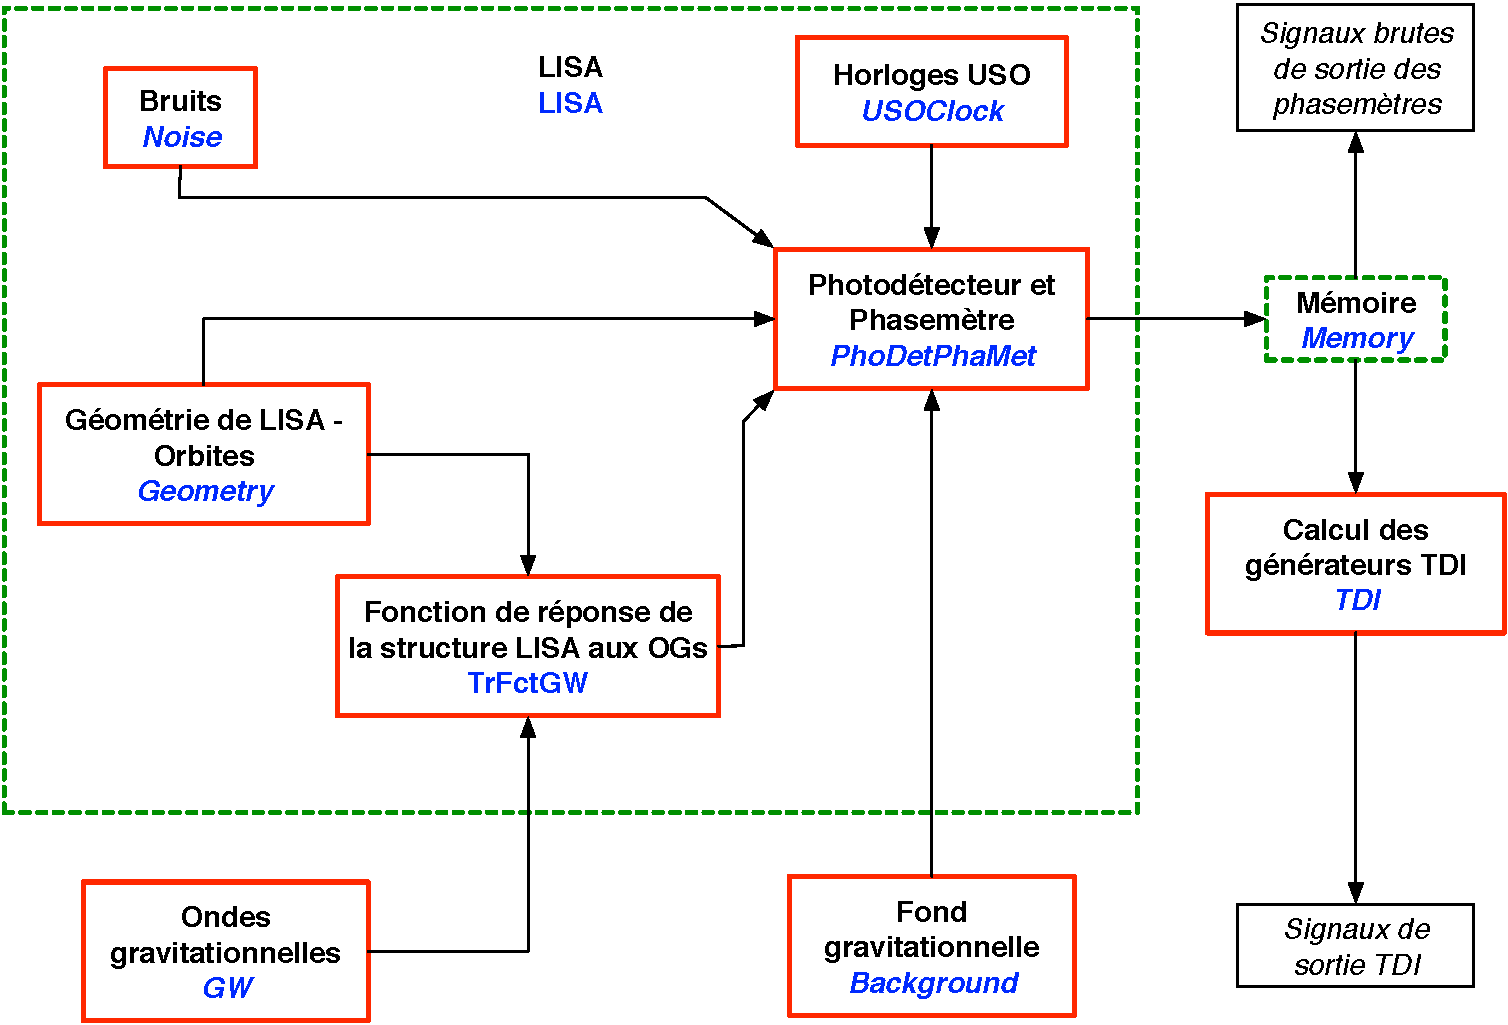
\includegraphics[width=14cm]{Figures/Structure.pdf}
\caption{\small Structure du simulateur LISACode. Les boites \textcolor{red}{rouge} repr\'esentent les modules principaux et les boites en \textcolor{green}{vert} les modules d'interface. Le nom g\'en\'erique des modules est en \textcolor{blue}{bleu}.\small} 
\label{Struct_LISACode}
\end{figure}

Il y a 9 modules : 
\begin{itemize}
\item {\em Outils\_Maths} : Objets utilis\'es comme outils par le programme : vecteurs, filtres, ...
\item {\em Ondes\_Gravit} : Mod\'elisation \textbf{OG} (monochromatique, binaire, quelconque).
\item {\em Orbitographie} : Mod\'elisation des orbites des satellites.
\item {\em Bruits} : Mod\'elisation des bruits (bruit blanc, bruit filtr\'e et bruit lu dans un fichier).
\item {\em USO\_Temps} : Mod\'elisation des horloges ultra-stables.
\item {\em Memoire} : Gestion des m\'emoires pour les sorties de chaque satellite.
\item {\em Input\_Data} : Lecture du fichier de configuration du simulateur.
\item {\em Detecteur} : Modelisation du d\'etecteurLISA : R\'eponse des bras aux ondes gravitationnelles, fonction de r\'eponse du phasem\`etre, interface et  avancement temporel.
\item {\em TDI} : Application des g\'en\'erateur TDI.
\end{itemize}

La figure \ref{Org_LISACode} montre l'organisation des biblioth\`eques utilis\'ees par LISACode. \\

\begin{figure}[!h]
\centering 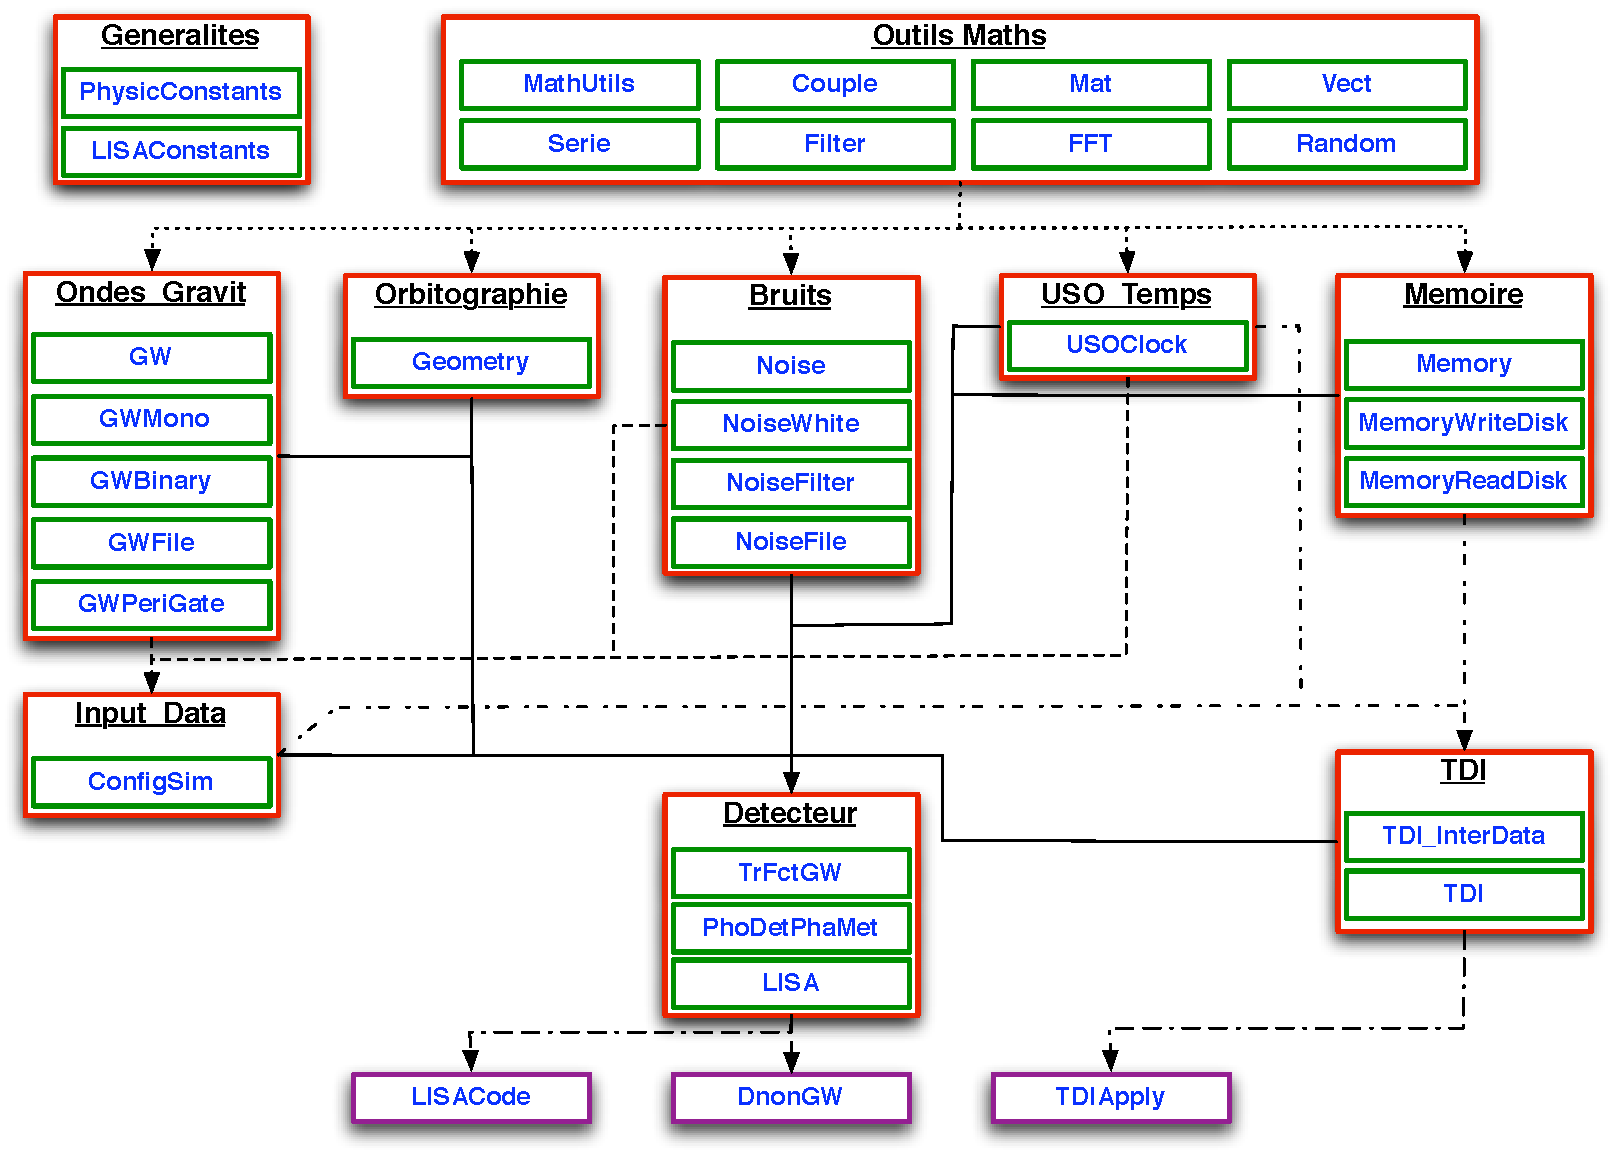
\includegraphics[width=15cm]{Figures/OrgPackage.pdf}
\caption{\small Organisation et d\'ependance  des biblioth\`eques du simulateur. Les cadres en \textcolor{green}{verts} repr\'esentent les objets, en  \textcolor{red}{rouge}  les biblioth\`eques et  en \textcolor{pink}{violet}, les executables. \small} 
\label{Org_LISACode}
\end{figure}

La premi\`ere entr\'ee est les OG. Elles peuvent �tre d\'efinie en interne gr\^ace \`a diff\'erents mod\`eles qui produisent des signaux issues de sources monochromatiques, de syst\`eme binaires avec une fr\'equence fix\'ee ou de syst\`eme binaire calcul\'e dans l'approximation Post-Newtoniennne (1 or 2.5 PN). L'OG peut \'egalement \^etre entr\'e via une s\'equence temporellequi provient par exemple de code de simulation plus sophistiqu\'e. \\

Les orbites de LISA sont g\'en\'er\'es en interne par le code. Ils correspondent \`a des orbites r\'ealistes qui prennent en compte tant la respiration et la rotation de LISA que le mouvement autour du Soleil. Les param\`etres de ces orbites peuvent \^etre ajust\'ees pour modifier la distance moyenne entre satellites ($5 \times 10^{9} \; m$ nominalement) ou pour fixer LISA \`a une certaine position. La position initial peut aussi \^etre d\'efinie en entr\'ee.\\

Un ingr\'edient important de la r\'eponse de LISA et par cons\'equent des codes est la sp\'ecification de bruits de diff\'erente nature. Cela inclut le bruit optique du au \emph{shot noise} aux \'el\'ements d\'ecris dans le taleau \ref{table_error}. Le bruit des masses inertielles et le bruit laser peuvent aussi \^etre d\'efinis en entr\'ee. Normalement, ces bruits sont d\'efinis comme des bruits blancs dans une bande fr\'equentielle d\'efinie mais diff\'erentes formes peuvent \^etre utilis\'ees.
\begin{table}[htdp] 
\caption{Budget des erreurs bas\'e sur le tableau 4.1 du  \cite{PrePhaseAReport}.  
La quatri\`eme colonne donne les erreurs par d\'efaut utilis\'ees dans LISACode. Ces valeurs peuvent \^etre modifi\'ees par l'utilisateur. La d\'ependance fr\'equentielle de ces bruits et discut\'es dans \ref{SSSConfigGW}} 
\begin{center} 
\small
\begin{tabular}{|c|c|c|c|c|} 
\hline 
Source d'erreur & Erreur & LISACode & Entr\'e LISACode (unit\'e de $\delta \nu \over \nu $)  \\ 
\hline 
\multicolumn{4}{|c|}{Bruit de mesure}  \\ 
\hline 
Shot noise&$11\times 10^{-12} {\rm m.{Hz}^{-{1 \over 2}}}$&$11$ & \footnotesize$ 2.3 \times 10^{-19}\left(f\over 1 Hz \right) \left(L \over 5 \times 10^{9}{\rm m} \right) \sqrt{1 {\rm  W}\over P }.{Hz}^{-{1 \over 2}} $\small \\ 
\hline 
USO & $5 \times10^{-12} {\rm m.{Hz}^{-{1 \over 2}}}$& &  \\  
\cline{1-2} 
bruit r\'esiduel du laser&$5 \times 10^{-12} {\rm m.{Hz}^{-{1 \over 2}}}$& &  \\ 
\cline{1-2} 
Instabilit\'e du pointage &$10 \times10^{-12} {\rm m.{Hz}^{-{1 \over 2}}}$& $16.5$ & $3.49 \times 10^{-19} \left(f\over 1 Hz \right).{Hz}^{-{1 \over 2}}$\\ 
\cline{1-2} 
Mesure de phase et offset&$5\times10^{-12} {\rm m.{Hz}^{-{1 \over 2}}}$& &  \\ 
\cline{1-2} 
Effet de lumi\`ere diffus\'ee&$5\times10^{-12} {\rm m.{Hz}^{-{1 \over 2}}}$& &  \\ 
\cline{1-2} 
Autres effets&$8.5\times10^{-12} {\rm m.{Hz}^{-{1 \over 2}}}$& & \\ 
\hline 
\multicolumn{4}{|c|}{Bruits d'acc\'el\'eration}  \\ 
\hline 
Bruit des masses inertielles & $3 \times10^{-15}{\rm m.s^{-2}.{Hz}^{-{1 \over 2}}}$& $3 $ & $1.59 \times 10^{-24} \left( 1 Hz \over f\right).{Hz}^{-{1 \over 2}}$\\ 
\hline 
\end{tabular} 
\end{center} 
%\label{default} 
\label{table_error} 
\end{table}% 
\normalsize

La r\'eponse de LISA \`a des OGs est calcul\'ee en utilisant les orbites et la fluctuation relative de fr\'equence r\'esultante (unit\'es de $\Delta \nu \over \nu$) est en entr\'ee du Module Phasemetre. Celle-ci est combin\'e avec les diff\'erentes contribution de bruits pour produire le signal primaire des phasem\`etres qui est ensuite filtr\'e par un filtre elliptique. Ce filtre est un filtre passe-bas qui coupe les fr\'equences \`a la moiti\'e de la fr\'equence de mesure pour \'eliminer le repliement de sp\`ectre.  Dans un cas standard,le signal  primaire est \`a 0.5 Hz et la sortie, apr\`es filtrage, \`a 1 Hz. \\

Ce signal peut-\^etre sauvegard\'e dans un fichier et/ou trait\'e par le module TDI en utilisant les combinaisons TDI d\'efinis en entr\'ee. Une decription d\'etaill\'ee des g\'en\'erateur TDI est donn\'e par \cite{TDIVinet2} et \cite{TDITinto}. \\

La description du code ci-dessus est seulement un bref r\'esum\'e de ses capacit\'es.


\newpage

%%%%%%%%%%%
%  INSTALLATION  %
%%%%%%%%%%%
\section{Installation}
\label{SInstall}
\subsection{Syst\`eme requis}
\label{SSSystReq}
Ce programme peut s'installer sur un syst\`eme UNIX standard disposant d'un compilateur C++.\\
Il existe \'egalement un ex\'ecutable sous Windows (test\'e uniquement sous Windows XP).\\ 

%
%   UNIX
%
\subsection{Sous Unix, Linux, Mac OS X}
\label{SSInstallUNIX}
\subsubsection{Installation}
\label{SSSInstallUNIX}
L'installation se fait de la m\^eme mani\`ere qu'un progamme "standard" sous UNIX. Les instructions \`a suivre sont les suivantes : 
\begin{enumerate}
\item T\'el\'echarer le fichier lisacode-1.3.tar.gz\\ (sur le web : http://www.apc.univ-paris7.fr/Downloads/lisa/LISACode/ )\\ et d\'eplacer le fichier dans le r\'epertoire ({\it MyDirectory} dans l'exemple) o\`u vous souhaitez installer LISACode.
\item D\'ecompresser la fichier : \\
\hphantom{aaaaa}\texttt{tar xvzf lisacode-1.3.tar.gz }\\
\item Aller dans le r\'epertoire {\it LISA\_Sim\_Tdi} :\\
\hphantom{aaaaa}\texttt{cd MyDirectory/lisacode-1.3 }\\
\item Ex\'ecuter le script de configuration, {\it configure}, pour creer les {\it makefile} , en tapant : \\
\hphantom{aaaaa}\texttt{./configure}\\
Il est possible d'ajouter des options de compilation et de sp\'ecifier le r\'epertoire o\`u les ex\'ecutable seront install\'es (voir la partie \ref{SSSInstallConfig} ou le fichier {\it INSTALL} pour plus d'informations sur ces deux points techniques).
\item Ex\'ecuter le {\it makefile} pour compiler le code : \\
\hphantom{aaaaa}\texttt{make}
\item Si vous souhaitez installer le simulateur avec les ex\'ecutables de votre machine ou dans le r\'epertoire sp\'ecifi\'e, utilisez la commande : \\
\hphantom{aaaaa}\texttt{make install}
\end{enumerate}

Si le programme s'est install\'e normalement, 3 ex\'ecutables se trouvent dans un r\'epertoire {\it MyDirectory/lisacode-1.3/Main/Test}. Les 3 ex\'ecutables sont :
\begin{itemize}
\item {\em LISACode} : Le programme de simulation principal qui mod\'elise les ondes gravitationnelles,
les �passe� dans l'ensemble du d\'etecteur et applique la pr\'e-analyse TDI sur les donn\'ees de sortie.
\item {\em DnonGW} : Programme qui donne les variations relatives de fr\'equence des faisceaux induites par les seules ondes gravitationnelles.
\item {\em TDIApply} : Application de g\'en\'erateurs TDI sur des donn\'ees pr\'ealablement simul\'ees.
\end{itemize}

Si vous utilisez {\it make install} pour la compilation, les 3 executables sont aussi dans le r\'epertoire {\it bin} situ\'e avec les ex\'ecutable de votre ordinateurou dans le r\'epertoire sp\'ecifi\'e {\it MyExe/bin}. Ce r\'epertoire comprend aussi plusieurs ex\'ecutables de test.\\

Pour plus de praticit\'e, copiez les ex\'ecutables dans votre r\'epertoire de travail (le r\'epertoire o\`u vous souhaitez effectuer les simulations de LISA).


\subsubsection{Option d'installation}
\label{SSSInstallConfig}
Les diff\'erentes options d'installation possibles sont d\'etaill\'ees dans le fichier  {\it INSTALL} situ\'e dans {\it MyDirectory/lisacode-1.3}.\\

Les options de compilation doivent \^etre sp\'ecifi\'e au moment de la configuration. Apr\`es le \texttt{./configure}, \texttt{CXXFLAGS=} suivi des options de compilation entre guillemets.Par exemple, pour optimiser la compilation sous un PowerPCG5, l'option est {\it -O3 -fast} d'o\`u la commande suivante pour l'installation : \\
\hphantom{aaaaa}\texttt{./configure CXXFLAGS="-O3 -fast -Wno-deprecated"} \\ 

Il est \'egalement possible de sp\'ecifier le chemin du r\'epertoire dans lequel les ex\'ecutables seront install\'es lors du \texttt{make install}. Pour cela, taper \texttt{--prefix=} suivi du chemin du r\'epertoire entre guillemets. Par exemple, la commande pour la configuration sous PowerPCG5 avec les ex\'ecutables dans le r\'epertoire{\it MyExe} est :
\hphantom{aaaaa}\texttt{./configure CXXFLAGS="-O3 -fast -Wno-deprecated" --prefix="MyExe"} \\


\subsubsection{Test de fonctionnement}
\label{SSSTestFonctUNIX}
Pour tester le fonctionnement du simulateur, utilisez le fichier de configuration de r\'ef\'erence {\it ConfigRefBase} avec les instructions suivantes :\\
\begin{enumerate}
%\item Copier le fichier {\it ConfigRefBase} situ\'e dans le r\'epertoire {\it Main/Test} , dans le r\'epertoire d'installation (dans l'exemple : �\texttt{../chemin/du/repertoire/}�).
\item Se placer dans ce r\'epertoire d'installation.
\item Lancer le simulateur : {\it LISACode} suivi du nom du fichier de configuration puis de "123456" (graine du g\'en\'erateur al\'eatoire). \\
\hphantom{aaaaa}\texttt{./LISACode ConfigRefBase 123456}
\end{enumerate}
Le programme met entre  10 secondes et  15 minutes pour ex\'ecuter les 10 000 s de la simulation. L'affichage final est  : \\
\texttt{...}\\
\texttt{10000 s     \#0100 \%} \\
\hphantom{aaaaa}\texttt{ X = 9.41546278836602e-19}\\
\hphantom{aaaaa}\texttt{ Y = 9.73859038667986e-19}\\
\hphantom{aaaaa}\texttt{ Z = 9.28457478808582e-19}\\
\hphantom{aaaaa}\texttt{ AlphaMan = 6.41358600758029e-19}\\
\hphantom{aaaaa}\texttt{ Beta = 6.48014274920517e-19}\\
\hphantom{aaaaa}\texttt{  X2s1 = 8.97752170019294e-19}\\
\hphantom{aaaaa}\texttt{ X2s2 = 9.41500592699302e-19}\\
\hphantom{aaaaa}\texttt{ X2s3 = 8.16992767767782e-19}\\
\hphantom{aaaaa}\texttt{ P1 = 4.98540196959974e-19}\\
\hphantom{aaaaa}\texttt{ Zeta1 = 7.07135169910109e-20}\\
\texttt{Final time : 10001 s}\\
\texttt{End}\\


%
%   Windows
%
\subsection{Sous Windows}
\label{SWindows}
Il existe un ex\'ecutable de LISACode sous Windows qui a \'et\'e test\'e sous Windows XP.
\subsubsection{Installation}
\label{SSInstallWindows}
Il n'y a pas d'installation \`a proprement parler ; il suffit juste de r\'eccup\'erer le fichier {\it LISACode\_1\_3\_for\_Windows.zip}  \`a l'adresse : \\
 {\it http://www.apc.univ-paris7.fr/Downloads/lisa/LISACode/version-1.3/}.\\
 D\'ecompresser le fichier et ex\'ecuter l'ex\'ecutable LISACode.exe.
\subsubsection{Test de fonctionnement}
\label{SSSTestFonctWindows}
Il est possible de tester le fonctionnement du simulateur en utilisant un fichier de configuration de r\'ef\'erence  ({\it ConfigRefBase}) situ\'e dans le m\^eme r\'epertoire que l'ex\'ecutable. La proc\'edure \`a suivre est la suivante : \\
\begin{enumerate}
\item Ouvrir une console MS-DOS et se placer dans le r\'epertoire ou se trouve l'ex\'ecutable et le fichier de configuration {\it ConfigRefBase} (\texttt{cd ...} ).
\item Lancer le simulateur : {\it LISACode} suivi du nom du fichier de configuration  ({\it ConfigRefBase}) puis de "123456" (graine du g\'en\'erateur al\'eatoire) . \\
\hphantom{aaaaa}\texttt{LISACode.exe ConfigRefBase 123456}
\end{enumerate}
On doit obtenir les m\^emes r\'esultats que ceux du chapitre~\ref{SSSTestFonctUNIX}.



\newpage

%%%%%%%%%%%
%  USE LISACODE  %
%%%%%%%%%%%

\section{Utilisation de LISACode}
\label{SUse}
\subsection{Ex\'ecution du simulateur et des deux programmes annexes}
\label{SSExecution}
Le programme principal qui effectue toute la simulation (des ondes gravitationnelles \`a TDI) se nomme {\it \bf LISACode}. Pour configurer la simulation, ce programme lit les informations contenues dans un fichier de configuration dont le d\'etail est donn\'e au paragraphe suivant. L'adresse des fichiers de sortie est sp\'ecifi\'ee dans le fichier de configuration. Pour lancer la simulation la ligne de commande est : \\
\hphantom{aaa}\texttt{./LISACode fichier\_de\_configuration}\\
{\it(si l'ex\'ecutable est dans le r\'epertoire de travail)}\\
\hphantom{aaa}ou\\
\hphantom{aaa}\texttt{../chemin/du/repertoire/d/installation/LISACode fichier\_de\_configuration}  \\
{\it(si l'ex\'ecutable n'est pas dans le r\'epertoire de travail)}\\
Il existe deux autres ex\'ecutables qui lisent \'egalement les informations du fichier de configuration. Ces deux ex\'ecutables n'effectuent qu�une partie de la simulation : \\
\begin{itemize}
\item {\it \bf DnonGW} : Ce programme effectue le calcul de la variation relative de fr\'equence des faisceaux lasers arrivant sur chaque phasem\`etre en tenant uniquement compte des ondes gravitationnelles (sp\'ecifi\'ees dans le fichier de configurations). Il donne en sortie trois fichiers (dont le nom ne peut pas \^etre sp\'ecifi\'e) qui sont : \\
\begin{itemize}
\item {\it DnGW\_GW.txt} : Evolution temporelle du $h_+$ et du $h_\times$ des ondes gravitationnelles.
\item {\it DnGW\_Position.txt} : Evolution temporelle des coordonn\'ees \'ecliptiques des trois satellites.
\item {\it DnGW\_TDelay.txt} : Temps de parcours des faisceaux le long des bras.
\item {\it DnGW\_SigFctTrGW.txt} : Variation relative des faisceaux lasers externes arrivant sur chaque photodiode.
\end{itemize}
Les param\`etres temporelles de la simulation sont ceux sp\'ecifi\'es dans le fichier de configurations.\\

\item {\it \bf TDIApply} : Ce programme applique les g\'en\'erateurs TDI sp\'ecifi\'es dans le fichier de configuration, sur des fichiers de donn\'ees brutes (sortie des phasem\`etres). Le fichier de sortie contient (comme pour la simulation compl\`ete) l'\'evolution temporelle de chaque g\'en\'erateurs TDI. Le nom de ce fichier est celui sp\'ecifi\'e dans le fichier de configurations.
\end{itemize}


%%%%%%%%%%%%%%%
%  CONFIGURATION FILE  %
%%%%%%%%%%%%%%%

\section{Fichier de configuration}
\label{SSConfigFile}

% Generalites  
%%%%%%%%
\subsection{G\'en\'eralit\'es}
\label{SSConfGen}
Ce fichier contient toutes les information pour configurer le simulateur. Il y a deux types de fichier possibles : ASCII ou XML. Le fichier XML peut \^etre construit avec le logiciel d'interface graphique {\it LISA\_AutoGUI.jar}. Les tableaux \ref{table_paramTime} , \ref{table_paramPrecisionTDI}, \ref{table_paramOrbits}, \ref{table_paramDetector}, \ref{table_paramRecord}, \ref{table_paramGW}, \ref{table_paramNoise} , \ref{table_paramUSO} and \ref{table_paramTDI}  listent les param\`etres.
\begin{table}[p] 
\caption{Liste des param\`etres utilis\'es pour configurer la simulation dont le type est \textbf{Time}. }
\begin{center} 
\begin{tabular}{|p{3.cm}|p{8.cm}|c|p{1.in}|} 
\hline 
Nom & D\'etails & Unit\'es & Valeur standard  \\ 
\hline 
 StepPhysic & Pas de temps utilis\'e pour mod\'eliser des processus continu, avant filtrage. & secondes & 0.5 \\ 
\hline 
 StepMeasure & Pas de temps dans le fichier de sortie du signal des phasm\`etre, apr\`e filtrage. & secondes & 1 \\ 
\hline 
 Max & Dur\'ee totale de calcul. & secondes & de 1 s \`a an \\ 
\hline 
 DeltaTDIDelay & Erreur possible sur l'estimation des temps de parcours. & secondes & de 0 \`a 1e-5 \\ 
\hline 
 StepDisplay & Pas de temps de l'affichage de l'avancement (pour suivre la simulation). & secondes & de 100 \`a 1e6 \\ 
\hline 
\end{tabular} 
\end{center} 
\label{table_paramTime} 
\end{table}

\begin{table}[p] 
\caption{Liste des param\`etres utilis\'es pour configurer la simulation dont le type est \textbf{PrecisionTDI}. }
\begin{center} 
\begin{tabular}{|c|p{8.cm}|c|c|} 
\hline 
Nom & D\'etails & Unit\'es & Valeur standard   \\ 
\hline
 Interpolation & Type d'interpolation utilis\'e pour TDI &  & LAG 20 \\ 
\hline 
 TDIDelayApprox & Si ON, les retards utilis\'es dans TDI sont ajout\'es sinon sinon ils sont imbriqu\'es  & On/Off & Off \\ 
 \hline
\end{tabular} 
\end{center} 
\label{table_paramPrecisionTDI} 
\end{table}

\begin{table}[p] 
\caption{Liste des param\`etres utilis\'es pour configurer la simulation dont le type est \textbf{Orbits}. }
\begin{center} 
\begin{tabular}{|c|p{8.cm}|p{3.cm}|p{2.cm}|} 
\hline
Nom & D\'etails & Unit\'es & Valeur standard   \\ 
\hline
 Armlength & Longueur de bras nominal entre les satellites de LISA & m\`etres & 5e9 \\ 
\hline 
 StartTime & Temps de d\'epart qui d\'efini la position de LISA sur son orbite au d\'emarrage du calcul.  & secondes (de 0 \`a 1 an) & 0 \\ 
\hline 
 InitialRotation & Phase initial de la configuration du triangle de LISA (0 : satellite 1 en bas) & radians & 0 \\ 
\hline 
 Move & 0 : les satellites de LISA sont fix\'es , 1: orbites ARTEMIS, 2: orbites MLDC  & 0 / 1 / 2 & 1 \\ 
\hline 
 Order & Ordre du calcul des temps de vol : 0 - temps calcul\'e \`a partir des positions des satellites ,1 - effet Sagnac  , 2 - effet de relativit\'e g\'en\'erale.  & 0 / 1 / 2 & 2 \\ 
\hline 
\end{tabular} 
\end{center} 
\label{table_paramOrbits} 
\end{table}

\begin{table}[p] 
\caption{Liste des param\`etres utilis\'es pour configurer la simulation dont le type est \textbf{Detector}. }
\begin{center} 
\begin{tabular}{|p{3.cm}|p{1.in}|p{6.cm}|p{2.cm}|p{2.cm}|} 
\hline 
 \multicolumn{2}{|c|}{Nom} & D\'etails & Unit\'es & Valeur standard  \\ 
\hline
 \multicolumn{2}{|c|}{LaserPower} & Puissance laser.  & Watt & 1 \\ 
\hline 
\multicolumn{2}{|c|}{PhaMetFilter} & Active ou d\'esactive le filtre du phasem\`etre.  & On/Off & On \\ 
\hline 
 PhaMetFilter-Parameters  &  attnuation &  Att\'enuation du filtre & dB & 180 \\
 \hline
 PhaMetFilter-Parameters  &  oscillation &  Oscillations en bande passante du filtre  & dB & 0.1 \\ 
 \hline
 PhaMetFilter-Parameters  &  FactFmes-ForHighFreq & Factor pour la fr\'equence de transition haute ( fr\'equence de transition haute sur la fr\'equence de mesure) &  & 0.1 \\ 
 \hline
 PhaMetFilter-Parameters  & FactFmes-ForLowFreq & Factor pour la fr\'equence de transition basse (fr\'equence de transition basse sur la fr\'equence de mesure) &  & 0.3 \\ 
 \hline
\end{tabular} 
\end{center} 
\label{table_paramDetector} 
\end{table}

\begin{table}[p] 
\caption{Liste des param\`etres utilis\'es pour configurer la simulation dont le type est  \textbf{Records}. }
\begin{center} 
\begin{tabular}{|c|p{8.cm}|c|} 
\hline 
 Nom & D\'etails &  Valeur standard  \\ 
\hline
 SignalSC 1& D\'efini le nom du fichier de sortie qui contient les donn\'ees brutes des phasm\`etres du satellite 1.  &  SC1.txt \\ 
\hline
 SignalSC 2& D\'efini le nom du fichier de sortie qui contient les donn\'ees brutes des phasm\`etres du satellite 2.  &  SC2.txt \\
\hline
SignalSC 3& D\'efini le nom du fichier de sortie qui contient les donn\'ees brutes des phasm\`etres du satellite 3.  &  SC3.txt \\ 
\hline
Delay & D\'efini le nom du fichier de sortie qui contient les 6 temps de vol en secondes.  &  Delay.txt \\ 
\hline
Position & D\'efini le nom du fichier de sortie qui contient les coordonn\'ees \'ecliptique des 3 satellites en m\`etres.  &  Delay.txt \\ 
\hline
TDI & D\'efini le nom du fichier de sortie qui contient les flux de donn\'ees des g\'en\'erateurs TDI.  &  TDI.txt \\ 
\hline 
\end{tabular} 
\end{center} 
\label{table_paramRecord} 
\end{table}

\begin{table}[p] 
\caption{Liste des param\`etres utilis\'es pour configurer la simulation dont le type est  \textbf{GW} (voir la figure \ref{GWParameters} ) \textbf{Mono} d\'efini une onde monochromatique, \textbf{Binary} d\'efini un syst\`eme binaire avec une fr\'equence fix\'ee et \textbf{PostNewtonBinary} d\'efini un syst\`eme binaire qui est calcul\'e dans l'approximation Post-Newtonienne. }
\begin{center} 
\begin{tabular}{|p{33.mm}|p{13.mm}|p{65mm}|p{24.mm}|p{18.mm}|} 
\hline 
\textbf{GW Type} & \textbf{Nom} & \textbf{D\'etails} & \textbf{Unit\'es} & \textbf{Valeur standard}  \\ 
\hline
All & Bet &Latitude \'ecliptique (d\'eclination) de la direction de la source (du Sun \`a source) & degr\'ees & de -90 \`a 90 \\
\hline
All & Lam & Longitude \'ecliptique (d\'eclination) de la direction de la source (du Sun \`a source) & degr\'ees & de 0 \`a 360 \\
\hline
All & Psi & Polarisation de la source : angle angle entre le r\'ef\'erentiel d'observation et le r\'ef\'erentiel  de la source & degr\'ees & de 0 \`a 360  \\
\hline
\hline
Mono & f & Fr\'equence de la source & Hertz &   \\
\hline
Mono & hp & Amplitude de la composante $+$ . & rien &1e-21  \\
\hline
Mono & hc & Amplitude de la composante $\times$ . & rien &1e-21  \\
\hline
Mono & Phi0hp & Phase initiale de la composante $+$. & radians & 0 \`a $2 \pi$  \\
\hline
Mono & Phi0hc & Phase initiale de la composante $\times$. & radians & 0 \`a $2 \pi$  \\
\hline
\hline
Binary & M1 & Masse du premier objet & masse solaire&   \\
\hline
Binary & M2 &  Masse du second objet & masse solaire&  \\
\hline
Binary & forb & Fr\'equence orbital du syst\`eme binaire. & Hertz &  \\
\hline
Binary & inc & Inclination : angle between angular momentum and source's direction & degrees & de -90 \`a 90 \\
\hline
Binary & phi0 &Phase initial du syst\`eme binaire. & radians & 0 \`a $2 \pi$  \\
\hline
Binary & r & Distance  d\'etecteur -  source. & KiloParsec &  \\
\hline
PostNewtonBinary & M1 & Masse du premier objet & masse solaire&    \\
\hline
PostNewtonBinary & M2 & Masse du second objet & masse solaire&  \\
\hline
PostNewtonBinary & tcoal & Temps de coalescence (\`a 0 au d\'ebut de la simulation). & secondes &  \\
\hline
PostNewtonBinary & inc & Inclinaison : angle entre le moment angulaire et la direction de la source & degr\'ees & de -90 \`a 90 \\
\hline
PostNewtonBinary & phase & Phase initiale du syst\`eme binaire. & radians & 0 to $2 \pi$  \\
\hline
PostNewtonBinary & r & Distance  d\'etecteur -  source. & KiloParsec &  \\
\hline
\hline
PostNewtonBinary & type & Type de calcul Post-Newtonian : 1 pour 1 PN et 2 pour 2.5 PN. & 1 / 2 & 2 \\
\hline
PostNewtonBinary & omega0 & Phase Post-Newtonian arbitraire. & degr\'ees & 1 \\
\hline
PostNewtonBinary & taud0 & Phase Post-Newtonienne sur le d\'etecteur. &  & 10  \\
\hline
PostNewtonBinary & gw & Facteur Post-Newtonien. &  & 1 \\
\hline
\end{tabular} 
\end{center} 
\label{table_paramGW} 
\end{table}

\begin{figure}[p] 
\centering 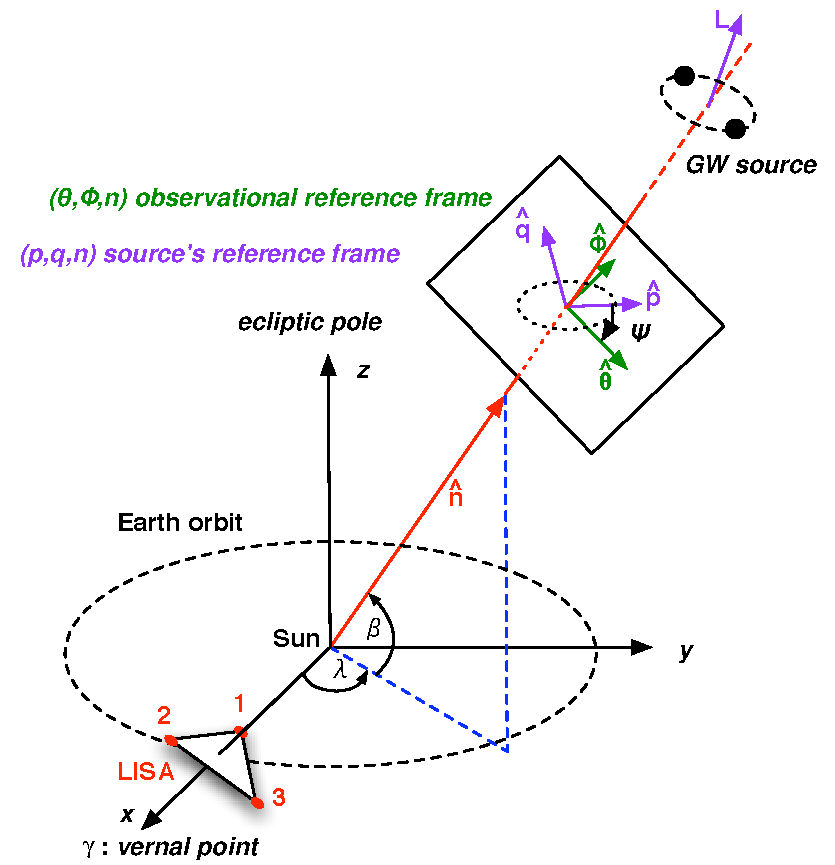
\includegraphics[width=10cm]{Figures/GWParameters.pdf} 
\caption{\small Description sch\'ematique des param\`etres de l'OG et des r\'ef\'erentiels.  La direction de la source est rep\'er\'e par la  d\'eclinaison $\beta$ et de la longitude \'ecliptique$\lambda$. ($ \widehat{\theta}$, $ \widehat{\phi}$, $\widehat{n}$) est le r\'ef\'erentiel observationnelle, i.e. le rep\`ere construit sur la direction de la source. Dans ce rep\`ere $ \widehat{\theta}$ est sur un m\'eridien. ($ \widehat{p}$, $ \widehat{q}$, $\widehat{n}$) est le r\'ef\'erentiel canonique .  
$\psi$ est l'angel de polarisation, i. e. l'angle entre le r\'ef\'erentiel canonique et le r\'efrentiel observationnel.} 
\label{GWParameters} 
\end{figure} 

\begin{table}[p] 
\caption{Liste des param\`etres utilis\'es pour configurer la simulation dont le type est  \textbf{Noise} (see figure \ref{SchBOSC1} for localization). }
\begin{center} 
\begin{tabular}{|p{22.mm}|p{20.mm}|p{65mm}|p{3.cm}|p{18.mm}|} 
\hline 
\textbf{Parameter type} & \textbf{Nom} & \textbf{D\'etails} & \textbf{Unit\'es} & \textbf{Valeur standard}  \\ 
\hline
Localization & Laser i j & \multicolumn{3}{|p{110.mm}|}{Bruit du laser associ\'e au banc optique du satellite i pointant vers le satellite i+1 si j = 0 et vers le satellite i-1 si j = 1. } \\
\hline
Localization & Mass i j & \multicolumn{3}{|p{110.mm}|}{ Bruit de la masse inertielle situ\'e dans le banc optique i j (i.e. banc optique du laser i j ). } \\
\hline
Localization & Shot i j & \multicolumn{3}{|p{110.mm}|}{ Shot noise du phasem\`etre qui mesure l'interf\'erence entre le faisceau du satellite distant le faisceau local du banc optique i j (i.e. banc optique du laser i j ). } \\
\hline
Localization & OOPN i j & \multicolumn{3}{|p{110.mm}|}{ Autres bruits sur le chemin optique situ\'e dans le banc optique i j (i.e. banc optique du laser i j ). } \\
\hline
Type & White  & Bruit blanc au niveau sp\'ecifi\'e. & ${\Delta \nu \over \nu} . Hz^{-1/2} $ unit & 1e-13 \\
\hline
Type & Filter\_1of  & Bruit filtr\'e en 1/f au niveau sp\'ecfi\'e. & ${\Delta \nu \over \nu} . Hz^{-1/2} $ unit & 1.59e-24 \\
\hline
Type & Filter\_f  &  Bruit filtr\'e en f au niveau sp\'ecifi\'e. & ${\Delta \nu \over \nu} . Hz^{-1/2} $ unit & 3.49e-19 \\
\hline
Type & Filter\_fLosP  & Bruit filtr\'e en f au niveau sp\'ecifi\'e proportionnel \`a la longueur des bras et  inversement proportionnelle \`a la racine carr\'ee de la puissance. & ${\Delta \nu \over \nu} . Hz^{-1/2} $ unit & 2.30e-19 \\
\hline
Type & FilterCoef  & Bruit filtr\'e o\`u les coefficients du filtre sont sp\'ecifi\'e explicitement : & &  \\
 & - alpha & Coefficient reccursif  & &  \\
 & - beta & Coefficient direct & &  \\
 & - stabilization & Nombre de donn\'ees n\'ecessaire \`a la stabilisation du filtre & pas &  10000 \\ 
\hline
\end{tabular} 
\end{center} 
\label{table_paramNoise} 
\end{table}

\begin{figure}[p] 
\centering 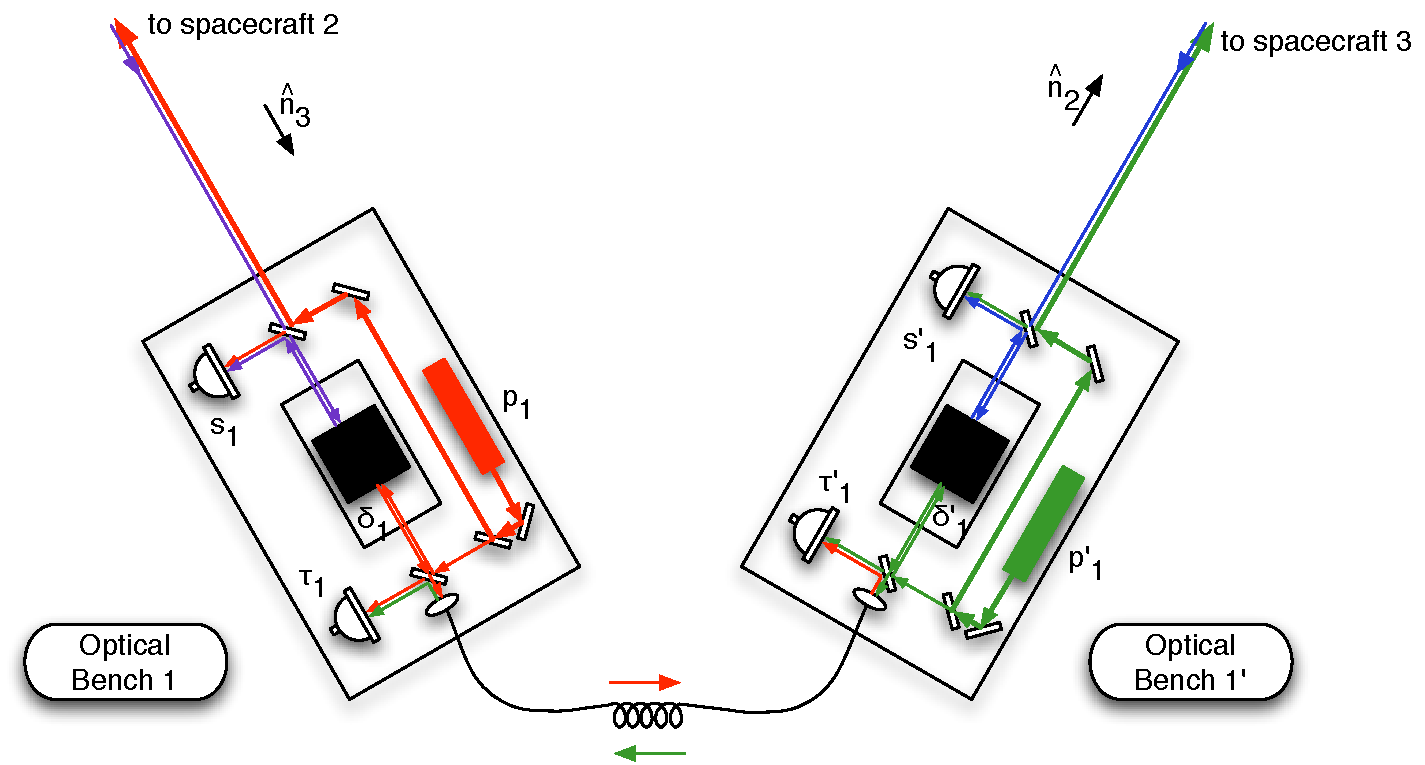
\includegraphics[width=10cm]{Figures/SchBOSC1.pdf} 
\caption{\small Repr\'esentation sch\'ematique des deux bancs optique du satellite 1.  
$s_{i}$ et$s'_{i}$ sont les phasem\`etres qui mesurent les interf\'erence entre le faisceau provenant du satellite distant et le faisceau du banc optique local, i.e. contenant le phasem\`etre. $\tau_{i}$ and $\tau'_{i}$ sont les phasem\`etres qui mesurentles interf\'erence entre les faisceaux de l'autre banc optique du m\^eme satellite et le faisceau du banc optique qui contient le phasem\`etre. $p$ est le laser et   
$\delta$ est la masse inertielle(formulation de \cite{TDITinto}).}   
\label{SchBOSC1} 
\end{figure}

\begin{table}[p] 
\caption{Liste des param\`etres utilis\'es pour configurer la simulation dont le type est  \textbf{USO}. Il y a un UltraStable Oscillateur par satellite specified by \textbf{SC} followed by the spacecraft number}
\begin{center} 
\begin{tabular}{|c|p{8.cm}|p{3.cm}|p{2.cm}|} 
\hline
Nom & D\'etails & Unit\'es & Valeur standard   \\ 
\hline
 offset & Offset de l'USO par rapport au temps courant & secondes & 0.006 \\ 
\hline
 derivs & Derive de l'USO par rapport au temps courant en seconde par seconde & secondes & 1e-7 \\ 
\hline
 noise & Bruit gaussien de l'USO par rapport au temps courant  avec le $\sigma$ sp\'ecifi\'e& secondes & 1e-7 \\ 
\hline
\end{tabular} 
\end{center} 
\label{table_paramUSO} 
\end{table}

\begin{table}[p] 
\caption{Liste des param\`etres utilis\'es pour configurer la simulation dont le type est  \textbf{TDI}. (\textbf{SC} satellite moyen)}
\begin{center} 
\begin{tabular}{|p{35.mm}|p{60.mm}|p{65.mm}|} 
\hline
Nom & D\'etails & Pack Value (in LISACode) \\ 
\hline
{\it Any name} & G\'en\'erateur TDI & \`a d\'efinir apr\`es le nom \\ 
\hline
X or Xf or X1s1 & Michelson premi\`ere g\'en\'eration centr\'e sur SC1 & 1 , 35 , 364 , 3653 , -4 , -53 , -521 , -5235  \\ 
\hline
Y or Yf or X1s2 & Michelson premi\`ere g\'en\'eration centr\'e sur SC2 & 2 , 16 , 145 , 1461 , -5 , -61 , -632 , -6316  \\ 
\hline
Z or Zf or X1s3 & Michelson premi\`ere g\'en\'eration centr\'e sur SC3 & 3 , 24 , 256 , 2542 , -6 , -42 , -413 , -4124  \\ 
\hline
X2 or Xf2 or X2s1 & Michelson seconde g\'en\'eration centr\'e sur SC1 & 1 , 35 , 364 , 3653 , 36524 , 365253 , 3652521 , 36525235 ,  -4 , -53 , -521 , -5235 , -52361 , -523635 , -5236364 , -52363653  \\ 
\hline
Y2 or Yf2 or X2s2 & Michelson seconde g\'en\'eration centr\'e sur SC2 & 2 , 16 , 145 , 1461 , 14635 , 146361 , 1463632 , 14636316 , -5 , -61 , -632 , -6316 , -63142 , -631416 , -6314145 , -63141461  \\ 
\hline
Z2 or Zf2 or X2s3 & Michelson seconde g\'en\'eration centr\'e sur SC3 & 3 , 24 , 256 , 2542 , 25416 , 254142 , 2541413 , 25414124 , -6 , -42 , -413 , -4124 , -41253 , -412524 , -4125256 , -41252542  \\ 
\hline
Alpha or alpha & G\'en\'erateur 1i\`ere g\'en\'eration $\alpha$ & -1 , -32 ,  -133 , 4 , 455 , 56  \\ 
\hline
Beta or beta & G\'en\'erateur premi\`ere g\'en\'eration $\beta$ & -121 , -2 , -13 , 64 , 5 , 566  \\ 
\hline
Gamma or gamma &G\'en\'erateur premi\`ere g\'en\'eration $\gamma$ & -21 , -232 , -3 , 464 , 45 , 6  \\ 
\hline
P1 & G\'en\'erateur Beacon sans faisceau re\'cu sur SC1 & 25 , -63 , -22 , 66 , 642 , -216 , 1463 , -1425  \\ 
\hline
Q1 & G\'en\'erateur Beacon sans faisceau re\'cu sur SC2 & 36 , -41 , -33 , 44 , 453 , -324 , 2541 , -2536  \\ 
\hline
R1 & G\'en\'erateur Beacon sans faisceau re\'cu sur SC3 & 14 , -52 , -11 , 55 , 561 , -135 , 3652 , -3614  \\ 
\hline
E1 & G\'en\'erateur Moniteur sans faisceau \'emis sur SC1 & 542 , 56 , -316 , -32 , -144 , 141 , 4 , -1  \\ 
\hline
F1 & G\'en\'erateur Moniteur sans faisceau \'emis sur SC2 & 653 , 64 , -124 , -13 , -255 , 252 , 5 , -2  \\ 
\hline
G1 & G\'en\'erateur Moniteur sans faisceau \'emis sur SC3 & 461 , 45 , -235 , -21 , -366 , 363 , 6 , -3  \\ 
\hline
U1 & G\'en\'erateur Relay sans faisceau de SC3 \`a SC1 et de SC1 \`a SC2 & 145 , 1464 , -5 , -64 , 16 , 2 , -6542 , -656  \\ 
\hline
V1 & G\'en\'erateur Relay sans faisceau de SC1 \`a SC2 et de SC2 \`a SC3 & 256 , 2545 , -6 , -45 , 24 , 3 , -4653 , -464  \\ 
\hline
W1 & G\'en\'erateur Relay sans faisceau de SC2 \`a SC3 et de SC3 \`a SC1 & 364 , 3656 , -4 , -56 , 35 , 1 , -5461 , -545  \\ 
\hline
\end{tabular} 
\end{center} 
\label{table_paramTDI} 
\end{table}


\newpage


% Configuration par fichier ASCII
%%%%%%%%%%%%%%%%%
\subsection{Configuration par fichier ASCII}
\label{SSConfACII}

LISACode peut lire les informations de configuration de la simulation dans un fichier de configuration ASCII. La syntaxe de ce fichier suit certaines r\`egles tr\`es strictes :
\begin{itemize}
\item \underline{\bf Toutes les lignes se terminent par un point virgule pr\'ec\'ed\'e d'un espace (� ;�)} que ce soit des lignes de commandes ou des lignes de commentaires.
\item Chaque bloc de caracteres doit etre separe du suivant par un espace.
\item Pour qu'une ligne soit en commentaire, il faut qu�elle commence par un "\#" suivi d'un espace.
\item C'est le premier mot d'une ligne (mot cl\'e principal) qui renseigne sur l'information que contient la ligne. Il existe 9 mots cl\'es principaux qui sont : \texttt{Time}, \texttt{Interpolation}, \texttt{TDIDelayApprox} , \texttt{Orbits}, \texttt{Detector}, \texttt{Record}, \texttt{GW}, \texttt{Noise}, \texttt{USO} et \texttt{TDI}. Le mot cl\'e principal est toujours suivi de ":".
\item La commande "END" stoppe la lecture du fichier de configuration.
\end{itemize}

% Configuration des temps
\subsubsection{Configuration des temps}
\label{SSSConfigTime}
Le mot cl\'e principal d'une ligne de configuration d'un param\`etre temporel est  \texttt{Time}. Une liste des parametres est donnee dans la tableau \ref{table_paramTime}. Les diff\'erents param\`etres temporels et les lignes les configurant sont :
\begin{itemize}
\item { \it Pas de temps physique} : C'est le pas de temps le plus petit de la simulation. Il correspond \`a la simulation des ph\'enom\`enes continus.\\
Ligne de configuration pour un pas de temps physique de 0.5 s : \\
\hphantom{aaaaa}\texttt{Time : StepPhysic 0.5 ;}  \\

\item { \it Pas de temps sur la prise de mesure } : C'est le pas de temps sur la prise des mesures par les phasem\`etres. Il correspond au pas de temps sur les donn\'ees de sortie et donc sur les resultats de TDI. \\
Ligne de configuration pour un pas de temps sur la prise de mesure de 1 s : \\
\hphantom{aaaaa}\texttt{Time : StepMeasure 1 ;}  \\ 

\item { \it Dur\'ee de la simulation } : C'est le temps que dure la simulation. \\
Ligne de configuration pour une simulation de 10000 s : \\
\hphantom{aaaaa}\texttt{Time : Max 10000 ;}  \\ 

\item { \it Impr\'ecision de l'information sur les temps de parcours} : Cette incertitude temporelle correspond \`a l'impr\'ecision sur la connaissance du temps de propagation le long des bras de LISA. C'est une erreur $\Delta D$ ajout\'ee sur les temps de parcours exacts $D_{real} = L_{real} / c$ avant leur utilisation par TDI. Les temps de parcours utilis\'es dans TDI $D_{TDI}$ sont donc : \\
\begin{equation}
D_{TDI} = D_{real} + \Delta D
\end{equation}
Ligne de configuration pour une impr\'ecision sur les retards de $10^{-6}$ s: \\
\hphantom{aaaaa}\texttt{Time : DeltaTDIDelay 1e-6 ;}  \\ 

\item { \it Pas de temps sur l'affichage} : Pas de temps sur l'affichage \`a l'\'ecran. Il permet a l'utilisateur de suivre l'evolution de la simulation.\\
Ligne de configuration pour un pas de temps d'affichage de 1000  s: \\
\hphantom{aaaaa}\texttt{Time : StepDisplay 1000 ;}  \\ 
\end{itemize}

%  Configuration de l'interpolation
\subsubsection{Configuration de l'interpolation}
\label{SSSConfigInterpolation}
Le mot cl\'e principal d'une ligne de configuration de l'interpolation est  \texttt{Interpolation}.   Il existe pour l'instant un seul type d'interpolation : l'interpolation lagrangienne
\begin{itemize}
\item { \it Interpolation dans l'application de TDI } : C'est le type d'interpolation faite sur les donn\'ees brutes de sorite des phasemetres lors de l'application des retards dans TDI. On interpole pour obtenir la valeur la plus realiste possible entre 2 mesures. Pour l'interpolation lagrangienne, on pr\'ecise l'ordre de l'interpolation.\\
Ligne de configuration pour d\'efinir l'interpolation dans l'application de TDI : \\
\hphantom{aaaaa}\texttt{Interpolation : LAG 20 ;}  \\
\end{itemize}

% Approximation des retards dans l'application de TDI
\subsubsection{Approximation des retards dans l'application de TDI}
\label{SSSConfigTDIQuick}
Il est possible d'accelerer le calcul de TDI en effectuant un calcul moins exact des retards. En effet lorsque l'on calcul le retard global a appliquer sur une mesure, il faut combiner les retards, en interpolant la valeur de chaque retard a partir des precedents. Par exemple le calcul normal d'un ''pack TDI'' est : 
\begin{equation}
D_{1} D_{2} D_{3} s_{2} = s_{2} \left( t - \left(  {L_{1}(t) \over c} + {L_{2} \left(t - {L_{1}(t) \over c} \right) \over c} + {L_{3}  \left( t - \left( {L_{1}(t) \over c} + {L_{2} \left(t - {L_{1}(t) \over c} \right) \over c} \right) \right) \over c}  \right)  \right)
\end{equation}
Lorsque l'on simplifie le calcul, les retards sont simplement pris a t et somm\'es sans interpolation. Soit pour l'example precedent :
\begin{equation}
D_{1} D_{2} D_{3} s_{2} = s_{2} \left( t - \left(  {L_{1}(t) \over c} + {L_{2}(t) \over c} + {L_{3}(t)  \over c}  \right)  \right)
\end{equation}
L'acceleration vient du fait que l'on a beaucoup moins d'interpolation a calculer.\\
\begin{itemize}
\item{\it Delay approximation} :  La ligne de configuration pour effectuer un calcul approximatif rapide de TDI est : \\
\hphantom{aaaaa}\texttt{TDIDelayApprox : off ;}  \\
\end{itemize}

% Configuration des orbites et du temps de parcours
\subsubsection{Configuration des orbites et du temps de parcours}
\label{SSSConfigOrbits}
Le mot cl\'e principal d'une ligne de configuration des orbites est  \texttt{Orbits}. Une liste des parametres est donnee dans la tableau \ref{table_paramOrbits}.
\begin{itemize}

\item { \it Longueur des bras } : Sp\'ecifie la longueur nominal des bras de LISA.\\
Ligne de configuration pour d\'efinir une longueur de bras nominal de $5 \times 10^{9} m$ : \\
\hphantom{aaaaa}\texttt{Orbits : Armlength 5e9 ;}  \\

\item { \it Temps initial des orbites } : Ce param\`etre temporel permet de d\'emarrer la simulation avec une position des satellites diff\'erentes de la configuartion de base. La configuration de base corresponds au position du tableau  \ref{table_flexing} soit le satellite 1 sur l'axe x et en dessous du plan de l'\'ecliptique et satellite 2 et 3 au dessus avec 2 en $y < 0$ et 3 en $y > 0$.\\
Ligne de configuration pour d\'efinir un temps de d\'emarrage des orbites de $5 \times 10^{6} s$ apr\`es la configuration initiale : \\
\hphantom{aaaaa}\texttt{Orbits : StartTime 5e6 ;}  \\

\item { \it Phase initial de rotation du triangle } : Ce param\`etre temporel permet de changer la position au temps 0 des satellites (temps courant  + temps initial des orbites) par rapport a la configuration de base definie dans la tableau \ref{table_flexing}. Elle correspond a un angle (en radians) de rotation dans le plan par rapport a la configuration de base. \\
Ligne de configuration pour d\'efinir un angle de rotation de $ \pi / 6$ par rapport a la configuration de base : \\
\hphantom{aaaaa}\texttt{Orbits : InitialRotation 0.523598776 ;}  \\

\item { \it Mouvement des satellites } : Ce param\`etre permet de mettre en mouvement ou non les satellites de LISA ainsi que de choisir le type d'orbites. On met \texttt{0} pour fixer les satellites, \texttt{1} pour les mettre en mouvement selon les orbites d\'efini par le laboratoire ARTEMIS \cite{OrbitLISA} et \texttt{2} pour les mettre en mouvement selon les orbites d\'efini par le Mock LISA Data Challenge \cite{SyntheticLISA}.\\
Ligne de configuration pour d\'efinir une simulation avec LISA mobile : \\
\hphantom{aaaaa}\texttt{Orbits : Move On ;}  \\

\item { \it Ordre dans le calcul des temps de propagation } : Ce param\`etre sp\'ecifie la precision avec lequel est fait le calcul du temps de parcours des photons entre satellites. Le parametre est a 0 pour un calcul classique considerant uniquement la distance entre satellite. Il est a1 pour un calcul tenant compte de l'effet Sagnac du a la rotation du trianlge c'est-a-dire que le long d'un meme bras les temps parcours different. Il est 2 pour un calcul tenant compte des effets de la relativit\'e g\'en\'erale. Si les satellites sont fixes (\texttt{Move Off}), on ne peut pas sp\'ecifier un autre ordre que 0.\\
Ligne de configuration pour d\'efinir un calcul relativiste des temps de propagation : \\
\hphantom{aaaaa}\texttt{Orbits : Order 2 ;}  \\
\end{itemize}

\begin{table}[!ht] 
\caption{Orbits basic configuration : Position, X, Y, Z (in meters) of the three spacecraft at different times  
(in seconds) for a nominal armlength of $5$ $10^6$ km.} 
\begin{center} 
\begin{tabular}{|c|c|c|c|c|} 
\hline 
Time of year (sec)&0& 7865000& 15730�000& 23595000 \\ 
\hline 
$X_1$& 148139203885 & -2145093689 & -151008051907 & -5067293342 \\ 
\hline 
$Y_1$& 0 &149589286122 & 1447675865 & -149546915581 \\ 
\hline 
$Z_1$& -2467045747 & 35723456 & 2514822292 & 84388495\\ 
\hline 
$X_2$& 150301280330 & 2186867586 & -148868371398 & -748229640 \\ 
\hline 
$Y_2$& -2478588950 & 148328221452 & -1034018214 & -150818789722\\ 
\hline 
$Z_2$& 1287273238 & -2121040808 & -1224681458 & 2168940029\\ 
\hline 
$X_3$& 150301280330 & 2150754223 & -148843921432 & -760789288 \\ 
\hline 
$Y_3$& 1287273238 & 150818900689 & 3970806949 & -148327868749\\ 
\hline 
$Z_3$&1286809645& 2193080836 & -1182122299 & -2145580218\\ 
\hline 
\end{tabular} 
\end{center} 
\label{table_flexing} 
\end{table}

% Configuration du detecteur
\subsubsection{Configuration du detecteur}
\label{SSSConfigDetector}
Le mot cl\'e principal d'une ligne de la configuration du d\'etecteur est  \texttt{Detector}. Cette configuration concerne des \'el\'ements sp\'ecifiques du d\'etecteur comme la puissance laser ou le filtre du phasem\`etre. Une liste des parametres est donnee dans la tableau \ref{table_paramDetector}.
\begin{itemize}
\item { \it Puissance Laser } : Sp\'ecifie la puissance des faisceaux \`a la sortie des lasers.\\
Ligne de configuration pour d\'efinir une puissance de laser de $1\;  Watt$ : \\
\hphantom{aaaaa}\texttt{Detector : LaserPower 1 ;}  \\

\item { \it Filtre du phasem\`etre} : Sp\'ecifie si on filtre ou non les signaux dans les phasem\`etres par un filtre passe-bas elliptique s'adaptant au pas de temps physique et au pas de temps de mesure. Ce filtre evite un repliement de spectre lors du sous-echantillonnage. On met \texttt{Off} pour rendre le filtre inactif et \texttt{On} pour le rendre actif. \\
Ligne de configuration pour fitrer les signaux dans le phasem\`etre : \\
\hphantom{aaaaa}\texttt{Detector : PhaMetFilter On ;}  \\

\item { \it Parametrisation du filtre elliptique du phasemetre} : Il y 4 parametres pour definir le filtre du phasemetre : l'attenuation en decibels caracterisee par le mot-cle \texttt{attenuation}, l'oscillation en bande passante  en decibels caracterisee par le mot-cle \texttt{oscillation}, la frequence de coupure haute definie comme un facteur (inferieur a 1) de la frequence de mesure caracterisee par le mot-cle \texttt{FactFmesForHighFreq} et la frequence de coupure basse definie comme un facteur (inferieur a 1) de la frequence de mesure caracterisee par le mot-cle \texttt{FactFmesForLowFreq}.\\
Ligne de configuration pour un filtre (filtre par defaut) d'attenuation de 180 dB , d'oscillation en bande passante de 0.1 dB, de frequence de coupure haute egal a 0.1 fois la frequence de mesure et de frequence de coupure basse egal a 0.3 fois la frequence de mesure : \\
\hphantom{aaaaa}\texttt{Detector : PhaMetFilterParameters : attenuation 180 oscillation 0.1 FactFmesForHighFreq 0.1 FactFmesForLowFreq 0.3 ;}  \\
\end{itemize}

% Output record configuration
\subsubsection{Configuration des fichiers de sorties}
\label{SSSConfigRecord}
Le mot cl\'e principal d'une ligne de configuration d'un fichier de sortie est \texttt{Record}. Il existe 4 types de fichiers de sortie. Les sorties pour lesquels aucun fichier n'est sp\'ecifi\'e ne sont pas enregistr\'es mais cela n'emp\^eche pas l'ex\'ecution du programme. Une liste des parametres est donnee dans la tableau \ref{table_paramRecord}.
\begin{itemize}
\item { \it Fichier de sortie des donn\'ees d'un satellite } : Fichier dans lequel sont stock\'ees les donn\'ees en sortie des 4 phasem\`etres d'un satellite. Ce fichier comporte 5 colonnes (voir la figure \ref{SchBOSC1} pour la position des phasemetres) : temps , phasemetre $s_{i}$ , phasemetre $s'_{i}$ , phasemetre $\tau_{i}$ , phasemetre $\tau'_{i}$.\\
Ligne de configuration pour d\'efinir l�enregistrement de la sortie du satellite 1 dans le fichier de nom "{\it SigPhaMetSC1.txt} " :\\
\hphantom{aaaaa}\texttt{Record : SignalSC 1 SigPhaMetSC1.txt ;}  \\
\item { \it Fichier d'enregistrement des temps de parcours } : Fichier dans lequel sont stock�es les 6
temps de parcours entre satellites. Ce fichier comporte 7 colonnes : temps , 3 temps de parcours dans le sens direct  ($L_{1} / c$  $L_{2} / c$ $L_{3} / c$) ,  3 temps de parcours dans le sens indirect ($L'_{1} / c$  $L'_{2} / c$ $L'_{3} / c$).\\
Ligne de configuration pour d\'efinir l'enregistrement des temps de parcours dans le fichier de nom  "{\it DelayTDI.txt} " : \\
\hphantom{aaaaa}\texttt{Record : Delay DelayTDI.txt ;}  \\

\item { \it Fichier d'enregistrement des positions des satellites} : Fichier dans lequel sont stock�es les 3 coordonn\'ees cartesiennes dans le referentiel eclipique des satellites. Ce fichier comporte 10 colonnes : temps , $x_{1}$ , $x_{2}$ , $x_{3}$ , $y_{1}$ , $y_{2}$ , $y_{3}$ , $z_{1}$ , $z_{2}$ , $z_{3}$ .\\
Ligne de configuration pour d\'efinir l'enregistrement des positions dans le fichier de nom  "{\it SCPos.txt} " :\\
\hphantom{aaaaa}\texttt{Record : Position SCPos.txt ;}  \\

\item { \it Fichier d'enregistrement des g\'en\'erateurs TDI } : Fichier dans lequel sont stock\'ees les r\'esultats des g\'en\'erateurs TDI sp\'ecifi\'es (voir \ref{SSSConfigTDI}). Ce fichier comporte une colonne pour le temps + une colonne par g\'en\'erateur TDI sp\'ecifi\'e.\\
Ligne de configuration pour d\'efinir l'enregistrement g\'en\'erateurs TDI dans le fichier de nom :  "{\it SignalTDI.txt} " : \\
\hphantom{aaaaa}\texttt{Record : TDI SignalTDI.txt ;}  \\
\end{itemize}

% Configuration des ondes gravitationnelles
\subsubsection{Configuration des ondes gravitationnelles}
\label{SSSConfigGW}
Le mot cl\'e principal d'une ligne de configuration d'une onde gravitationnelle est \texttt{GW}.  Une liste des parametres est donnee dans la tableau \ref{table_paramGW}.  More scientific information on LISACode gravitational waves are available in article of A.Petiteau \cite{LISACode}. Il existe 4 types d'onde gravitationnelle possibles dans le simulateur. Chaque param\`etre est d\'efini, en pr\'ec\'edent la valeur, d'un mot cl\'e correspondant au param\`etre. Pour tous les types d'onde, on pr\'ecise juste apr\`es "\texttt{GW}", la direction de la source en coordonn\'ees \'ecliptiques ($\beta \in \left[ -90^{o} , 90^{o} \right] \rightarrow$ \texttt{\{Bet\}}, $\lambda \in \left[ 0^{o} , 360^{o} \right] \rightarrow$ \texttt{\{Lam\}}) et l'angle de polarisation $\Psi \in \left[ 0^{o} , 360^{o} \right] \rightarrow$ \texttt{\{Psi\}}. Ces 3 angles sont schematise sur la figure \ref{GWParameters}.  Attention ils sont d\'efinis en degr\'ees. Par exemple pour une onde dont la source est \`a $\beta = 27^{o}$ et $\lambda = 297^{o}$ et dont l'angle de polarisation $\psi = 229^{o}$, le d\'ebut de la ligne de configuration est : \\
\hphantom{aaaaa}\texttt{GW : Bet 27.0 , Lam 297.0 , Psi 229.0 : ... ;}  \\

\begin{itemize}
\item { \it Onde gravitationnelle monochromatique } \texttt{\{Mono\}} : Onde gravitationnelle monochromatique dont on d\'efinit la fr\'equence \texttt{\{f\}}, l'amplitude de chaque composante de polarisation ($h_{+0}$ \texttt{\{hp\}} et $h_{\times 0} $ \texttt{\{hc\}}) et la phase initiale (en radians) de chaque composante de polarisation($\Phi_{+0}$ \texttt{\{Phi0hp\}} et $\Phi_{\times 0} $ \texttt{\{Phi0hc\}}). L'evolution temporelle des contraintes gravitationnelles de l'onde dans le referentiel propre de l'onde (CFR : Canonical Reference Frame) ${h}_{CFR+} (t)$ et ${h}_{CFR\times} (t)$ correspond a :
\begin{equation} 
\left\{ \begin{array}{lll}  
{h}_{CFR+} (t) & = & h_{0+}  \sin \left( 2 \pi f t + \phi_{0+}\right)\\ 
h_{CFR\times} (t) & = & h_{0\times}  \sin \left( 2 \pi f t + \phi_{0\times}\right) 
\end{array} \right.  
\label{GWMono} 
\end{equation}

Ligne de configuration pour d\'efinir une onde gravitationnelle monochromatique dont la direction de la source est $\beta = 50^{o}$ et $\lambda = 230^{o}$, l'angle de polarisation $\psi = 15^{o}$, la fr\'equence $f=10^{-4}$, l'amplitude des composantes $h_{+0}=10^{-21}$ et $h_{\times0}=0$ et la phase initiale des composantes de polarisation $\Phi_{+0} = 0$ et $\Phi_{\times 0} = 0$ :\\
\hphantom{aaaaa}\texttt{GW : Bet 50 , Lam 230 , Psi 15 : Mono : f 1e-4 , hp 1e-21 , hc 0.0 , Phi0hp 0.0 , Phi0hc 0.0 ;}  \\

\item { \it Onde gravitationnelle d'une binaire de fr�quence fix�e } \texttt{\{Binary\}} : Onde gravitationnelle issue d'une source binaire de fr�quence fix�e pour laquelle on d\'efinit les masses des deux astres $m_{1}$ \texttt{\{M1\}} et $m_{2}$ \texttt{\{M2\}} en masse solaire, la fr\'equence orbitale $f_{orb}$ \texttt{\{forb\}} en Hz, l'angle d�inclinaison $i$ \texttt{\{inc\}} en degrees, la phase initiale $\phi_{0}$ \texttt{\{Phi0\}} entre $0$ et $2\pi$ et la distance entre la source et le d\'etecteur $r$ \texttt{\{r\}} en kpc. L'evolution temporelle des contraintes gravitationnelles de l'onde dans le referentiel propre de l'onde (CFR : Canonical Reference Frame) ${h}_{CFR+} (t)$ et ${h}_{CFR\times} (t)$ correspond a : 
\begin{equation} 
\left\{ \begin{array}{lll}  
h_{CRF+} &=& A \left(1 + \cos^2 i \right) \cos \left( 4 \pi f_{orb} t + \phi_0 \right)\\ 
h_{CRF\times} &=& -2 A \cos i  \sin \left( 4 \pi f_{orb} t + \phi_0 \right) 
\end{array} \right.  
\label{GWBinaryFixedFreq} 
\end{equation} 
avec 
\begin{eqnarray} 
m_{tot} &=& m_1 + m_2 \label{mtot}\\ 
R &=& {\left( { G m_{tot} \over {\left( 2 \pi f_{orb} \right)}^2} \right)}^{1/3} \label{RBinFixF}\\ 
A &=& {2 G^2 \over c^4} {m_1 m_2 \over R r} \label{ABinFixF} 
\end{eqnarray}

Ligne de configuration pour d\'efinir une onde gravitationnelle issue d'une binaire de direction $\beta = 37.34^{o}$, $\lambda= 350^{o}$, l�angle de polarisation $\psi = 141.06^{o}$, de masses $M1 = 0.5 M_S$ et $M2 = 0.033 M_S$ , de fr\'equence f$ = 9.72044 \times 10^{-4}$, d'inclinaison $i = 88^{o}$, de phase initiale $\psi_0 = 0^{o}$ et de s\'eparation $r = 0.1$ kpc : \\
\hphantom{aaaaa}\texttt{GW : Bet 37.34 , Lam 350 , Psi 141.06 : Binary : M1 0.5 , M2 0.033 , forb 9.72044e-4 , inc 88 , phi0 0 , r 0.1 ;}  \\

\item { \it Onde gravitationnelle d'une binaire de fr�quence fix�e } \texttt{\{PostNewtonBinary\}} : Onde gravitationnelle issue d'une source binaire calculee dans l'approximation Post- Newtonienne a 1 PN ou 2.5 PN  pour laquelle on d\'efinit les masses des deux astres $m_{1}$ \texttt{\{M1\}} et $m_{2}$ \texttt{\{M2\}} en masse solaire, le temps de coalescence  $t_{coal}$ \texttt{\{tcoal\}} en seconds, l'angle d'inclinaison $i$ \texttt{\{inc\}} en degrees, la phase initiale $\phi_{0}$ \texttt{\{Phi0\}} entre $0$ et $2\pi$ et la distance entre la source et le d\'etecteur $r$ \texttt{\{r\}} en kpc. L'ordre Post-Newtonien du calcul est de 1 PN lorsque le parametre \texttt{\{type\}} est a 1 ou de 2.5 PN lorsque le parametre \texttt{\{type\}} est a 2. Pour le calcul a 2.5 PN, il faut preciser 3 parametres qui sont : une phase initial arbitraire \texttt{\{omega0\}}, la phase a l'entree du detecteur \texttt{\{taud0\}} et un parametre Post-Newtonien\texttt{\{gw\}}  egal a 1 dans la plupart des cas. Le calcul de l'evolution temporelle des contraintes gravitationnelles de l'onde dans le referentiel propre de l'onde (CFR : Canonical Reference Frame) ${h}_{CFR+} (t)$ et ${h}_{CFR\times} (t)$ est base sur des articles \cite{2PN_1}, \cite{2PN_2}, \cite{2PN_3} et  \cite{2PN_4}\\
Ligne de configuration pour d\'efinir une onde gravitationnelle issue d'une binaire de direction $\beta = 37.34^{o}$, $\lambda= 350^{o}$, l�angle de polarisation $\psi = 141.06^{o}$, de masses $M1 = 0.5 M_S$ et $M2 = 0.033 M_S$ , de fr\'equence f$ = 9.72044 \times 10^{-4}$, d'inclinaison $i = 88^{o}$, de phase initiale $\psi_0 = 0^{o}$ et de s\'eparation $r = 0.1$ kpc : \\
\hphantom{aaaaa}\texttt{GW : Bet 37.34 , Lam 352.0 , Psi 141.06  : PostNewtonBinary : M1 1.0e6 , M2 1.0e6 , tcoal 9676800.0 , inc 90 , phase 1.2 , r 1e5 , type 2 , omega0 1.0 , taud0 10.0 , gw 1.0 ;}  \\

\item { \it Onde gravitationnelle quelconque (lecture d'un fichier)} \texttt{\{File\}} : Onde gravitationnelle quelconque dont l'\'evolution temporelle des composantes de polarisation est lue dans un fichier (3 colonnes : $temps \; \; h_+ \; \; h_{\times} $).\\
Ligne de configuration pour d\'efinir une onde gravitationnelle lue dans le fichier {\it GWFile.txt} dont la direction de la source est $\beta = 50^{o}$ et $\lambda = 230^{o}$ et l'angle de polarisation $\psi = 15^{o}$. \\
\hphantom{aaaaa}\texttt{GW : Bet 50 , Lam 230 , Psi 15 : File : GWFile.txt ;}  \\
%\item { \it Onde gravitationnelle porte p\'eriodique} \texttt{[PeriGate]} : Onde gravitationnelle dont la forme des deux composantes h+ et hx , est une porte p�riodique. Cette forme non r\'ealiste d�onde gravitationnelle permet de balayer une large gamme de fr\'equence ($f << fmin$ ) et ainsi d'avoir la r\'eponse du d\'etecteur pour une direction de source donn\'ee. On d\'efinit \'egalement l'amplitude des deux composantes $h_{+0}$ et $h_{\times0}$. \\
%Ligne de configuration pour d\'efinir une onde porte p\'eriodique dont la direction de la source est $\lambda = 50^{o}$ et $\beta = 230^{o}$, l'angle de polarisation $\psi = 15^{o}$, la fr\'equence $f=10^{-5}$, l'amplitude des composantes $h_{+0}=1$ et $h_{\times0}=0$ :\\
%\hphantom{aaaaa}\texttt{GW : Lam 50 , Bet 230 , Psi 15 : PeriGate : f 1e-5 , hp 1 , hc 0 ;}  \\
\end{itemize}

% Configuration des bruits
\subsubsection{Configuration des bruits}
\label{SSSConfigGW}
Le mot cl\'e principal d'une ligne de configuration des bruits est \texttt{Noise}. Une liste des parametres est donnee dans la tableau \ref{table_paramNoise}. La configuration d'un bruit se fait ensuite en deux \'etapes : la localisation du bruit puis sa nature. La localisation du bruit se fait par le mot cl\'e correspondant \`a la situation du bruit : \texttt{Laser} pour le bruit issu d'un laser  - \texttt{Mass} pour le bruit sur une masse inertielle - \texttt{Shot} pour le bruit de "shot noise" - \texttt{OOPN} pour le bruit des autres bruits de chemin optique (autre que le "shot noise"). Le mot cl\'e de localisation est suivi du num\'ero du satellite (1, 2 et 3) puis le "sens" du banc : 0 si le banc est dans le "sens direct " ($1\rightarrow 3\rightarrow 2\rightarrow 1$), 1 s'il est dans le "sens indirect" ($1\rightarrow 2\rightarrow 3\rightarrow 1$). On sp\'ecifie ensuite la nature du bruit : \\
\begin{itemize}

\item { \it Bruit blanc }  \texttt{\{White\}}: Mod\'elisation d'un bruit blanc de densit\'e spectrale de puissance donn\'ee.\\
Ligne de configuration pour d\'efinir un bruit blanc de densit\'e spectrale de puissance $10^{-13}$ (sans dimension car exprim\'e en variation relative de fr\'equence) sur le laser du banc optique du satellite 1 en vis-\`a-vis avec le satellite 2 :\\
\hphantom{aaaaa}\texttt{Noise : Laser 1 0 : White 1.0e-13 ;}  \\

\item { \it Bruit filtr\'e pour une \'evolution en $1/f$ de l'amplitude (ou $\sqrt{PSD}$)} \texttt{\{Filter\_1of\}}: Mod\'elisation d'un bruit dont l'amplitude \'evolue en $1/f$. La seule valeur \`a sp\'ecifier est le niveau du bruit $A_{\delta \nu / \nu}$ en $Hz^{1/2}$  c'est-\`a-dire l'amplitude (ou $\sqrt{PSD}$) tel que $PSD_{\delta \nu / \nu} = A^2_{\delta \nu / \nu} f^{-2}$ . Les coefficients sont ensuite automatiquement calcul\'es par rapport au pas de temps\footnote{Les coefficients du filtre pour un bruit en $PSD_{\delta \nu / \nu} = A^2_{\delta \nu / \nu} f^{-2}$ sont : $\alpha_{1} = 1$ et $\beta_{0} = \beta_{1} = {A_{\delta \nu / \nu} \pi \Delta t} $ }.\\
Par exemple, le bruit d'une masse inertielle est generalement exprime comme un bruit d'acceleration en $m.s^{-2}.Hz^{-1/2}$: $\sqrt{S_{\Delta a , MI }} = 3 \times 10^{-15} m.s^{-2}.Hz^{-1/2}$ . Le calcul du $A_{\delta \nu / \nu , MI}$ est alors : 
\begin{equation}
A_{\delta \nu / \nu , MI} = {1 \over 2 \pi c} \sqrt{S_{\Delta a , MI }} = 1.59 \times 10^{-24} Hz^{1/2}
\end{equation}
Ligne de configuration pour d\'efinir un bruit de densit\'e spectrale de puissance $PSD_{\delta \nu / \nu} = \left( 1.59 \times 10^{-24} Hz^{1/2}\right)^2 f^{-2}$ sur les masses inertielles du banc optique du satellite 2 en vis-\`a-vis avec le satellite 1 : \\
\hphantom{aaaaa}\texttt{ Noise : Mass 2 1 : Filter\_1of 1.59e-24 ;} \\

\item { \it Bruit filtr\'e pour une \'evolution en $f$ de l'amplitude (ou $\sqrt{PSD}$)} \texttt{\{Filter\_f\}}: Mod\'elisation d'un bruit dont l'amplitude \'evolue en $f$. La seule valeur \`a sp\'ecifier est le niveau du bruit $A_{\delta \nu / \nu}$ en $Hz^{-3/2}$ c'est-\`a-dire l'amplitude (ou $\sqrt{PSD}$) tel que $PSD_{\delta \nu / \nu} = A^2_{\delta \nu / \nu} f^{2}$ . Les coefficients sont ensuite automatiquement calcul\'es par rapport au pas de temps\footnote{Les coefficients du filtre pour un bruit en $PSD_{\delta \nu / \nu} = A^2_{\delta \nu / \nu} f^{2}$ sont : $\alpha_{1} = -1$ , $\beta_{0} = {A_{\delta \nu / \nu} \over \pi \Delta t} $ et  $\beta_{1} = - {A_{\delta \nu / \nu} \over \pi \Delta t} $ }.
Par exemple, le bruit de chemin optique dans les bancs est generalement exprime comme un bruit  en $m.Hz^{-1/2}$ : $\sqrt{S_{\Delta a , OOPN }} = 16.7 \times 10^{-12} m.Hz^{-1/2}$ . Le calcul du $A_{\delta \nu / \nu , OOPN}$ est alors : 
\begin{equation}
A_{\delta \nu / \nu , OOPN} = {2 \pi \over  c} \sqrt{S_{\Delta a , OOPN}} = 3.49 \times 10^{-19} Hz^{-3/2}
\end{equation}\\
Ligne de configuration pour d\'efinir un bruit de densit\'e spectrale de puissance $PSD_{\delta \nu / \nu} = \left( 3.49 \times 10^{-19} Hz^{-3/2} \right)^2 f^{2}$ sur les bruits de chemin optique du banc optique satellite 3 en vis-\`a-vis avec le satellite 2 : \\
\hphantom{aaaaa}\texttt{Noise : OOPN 3 1 : Filter\_f 3.49e-19 ;} \\

\item { \it Bruit filtr\'e pour une \'evolution en $f$ de l'amplitude (ou $\sqrt{PSD}$), proportionnel \`a la longueur des bras et inversement proportionnel \`a la puissance laser} \texttt{\{Filter\_fLosP\}}: Mod\'elisation d'un bruit dont l'amplitude \'evolue en $f$ et est proportionnelle \`a la longueur des bras et inversement proportionnelle \`a la puissance laser. La seule valeur \`a sp\'ecifier est le niveau du bruit $A_{\delta \nu / \nu}$  en $Hz^{-3/2}$ c'est-\`a-dire l'amplitude (ou $\sqrt{PSD}$) tel que $PSD_{\delta \nu / \nu} = A^2_{\delta \nu / \nu} f^{2} {\left(L \over 5\times10^{9} \;m \right)}^2 \left(1 \; W \over P \right)$ . Les coefficients sont ensuite automatiquement calcul\'es par rapport au pas de temps\footnote{Les coefficients du filtre pour un bruit en  $PSD_{\delta \nu / \nu} = A^2_{\delta \nu / \nu} f^{2} {\left(L \over 5\times10^{9} \;m \right)}^2 \left(1 \; W \over P \right)$ sont : $\alpha_{1} = -1$ , $\beta_{0} = {A_{\delta \nu / \nu} \over \pi \Delta t}  {\left(L \over 5\times10^{9} \;m \right)} \sqrt{\left(1 \; W \over P \right)} $ et  $\beta_{1} = - {A_{\delta \nu / \nu} \over \pi \Delta t}  {\left(L \over 5\times10^{9} \;m \right)} \sqrt{\left(1 \; W \over P \right)} $ }.\\
Ligne de configuration pour d\'efinir un bruit de densit\'e spectrale de puissance $PSD_{\delta \nu / \nu} = \left( 2.30 \times 10^{-19} Hz^{-3/2}\right)^2 f^{2} {\left(L \over 5\times10^{9} \;m \right)}^2 \left(1 \; W \over P \right)$ sur le "shot noise" du banc optique satellite 3 en vis-\`a-vis avec le satellite 2 : \\
\hphantom{aaaaa}\texttt{ Noise : Shot 3 1 : Filter\_fLosP 2.30e-19 ;} \\

\item { \it Bruit filtr\'e quelconque}: Mod\'elisation d'un bruit filtr\'e quelconque d\'efini par les coefficients r\'ecursifs $\alpha$ \texttt{\{alpha\}} et directs $\beta$ \texttt{\{beta\}} du filtre \`a r\'eponse impulsionnelle infinie (IIR). On peut \'egalement pr\'eciser le temps n\'ecessaire � la stabilisation du filtre \texttt{\{stablization\}}. S'il y a plusieurs coefficients d�un m\^eme type, il faut les s\'eparer par des virgules.\\ \\
Ligne de configuration pour d\'efinir un bruit filtr\'e dont les coefficients du filtre sont $\alpha = \{1\}$ et $\beta = \{5\times10^{-24} , 5\times10{-24}\}$ (bruit d'acc\'el\'eration en $f^{-2}$ sur la densit\'e spectrale de puissance) sur la masse inertielle du banc optique du satellite 2 en vis-\`a-vis avec le satellite 1 : \\
\hphantom{aaaaa}\texttt{Noise : Mass 2 1 : FilterCoef : alpha 1.0 beta 5e-24 , 5e-24 ;}  \\ \\
Ligne de configuration pour d�finir un bruit filtr\'e dont les coefficients du filtre sont $\alpha = \{3.9939806575 , -5.9819996369 , 3.9820571154 , -0.9940381365\}$ et $\beta = $ $\{ 0.0000510993 ,$ $ -0.0002040002 , $ $ 0.0003058023 , $ $ -0.000204002 ,$ $ 0.0000510993 \} $ sur la masse inertielle du banc optique du banc optique du satellite 3 en vis-\`a-vis avec le satellite 2 (attention ce bruit n'a strictement aucune r\'ealit\'e physique et est juste pr\'esent\'e \`a titre d'exemple de syntaxe): \\
\hphantom{aaaaa}\texttt{Noise : Bench 3 1 : FilterCoef : alpha 3.9939806575 , -5.9819996369 , 3.9820571154 , -0.9940381365 beta 0.0000510993 , -0.0002040002 , 0.0003058023 , -0.000204002 , 0.0000510993 stablization 10000 ;}  \\

\item { \it Bruit lu dans un fichier }: Mod\'elisation d'un bruit \`a partir des valeurs d'un fichier ( 2 colonnes : temps bruit). Le programme charge l'ensemble des valeurs est commence \`a lire les valeurs � partir d'un point quelconque du fichier.\\
Ligne de configuration pour d\'efinir un bruit lu dans le fichier {\it NoiseOB.txt} et attribu\'e au banc optique du satellite 1 en vis-\`a-vis avec le satellite 2 : \\
\hphantom{aaaaa}\texttt{Noise : Laser 1 0 : File NoiseOB.txt ;}  \\
\end{itemize}

% USO
\subsubsection{Configuration des USOs}
\label{SSSConfigUSO}
Le mot cl\'e principal d'une ligne de configuration d'un oscillateur ultra-stable est \texttt{USO}. Une liste des parametres est donnee dans la tableau \ref{table_paramNoise}. Il faut tout d'abord d\'efinir le satellite auquel l'USO appartient : pour cela on pr\'ec\`ede le num\'ero du satellite du mot cl\'e SC. On peut ensuite d\'efinir 3 param\`etres pour un oscillateur ultra-stable (USO) :  un offset \texttt{[offset]} en seconde, une d\'erive dans le temps en seconde par seconde \texttt{[derivs]} et le $\sigma$ d'un bruit blanc gaussien \texttt{[noise]} en seconde. Ces param\`etres sont sp\'ecifi\'es en pr\'ec\'edent la valeur par le mot cl\'e correspondant. Si l'on ne d\'efinit pas un USO, celui-ci est suppos\'e parfait. \\
Ligne de configuration pour d\'efinir l'oscillateur du satellite 2 avec un offset de 0.006 s, une d\'erive de  $10^{-6} s.s^{-1}$ et un bruit de sigma $10^{-7} s$ : \\
\hphantom{aaaaa}\texttt{USO : SC 2 : offset 0.006 derivs 1e-6 noise 1e-7 ;} \\ \\


% Configuration de TDI
\subsubsection{Configuration de TDI}
\label{SSSConfigTDI}
Le mot cl\'e principal d'une ligne de configuration d'un g\'en\'erateur TDI est \texttt{TDI}. Le mot cl\'e est suivi du nom du g\'en\'erateur puis de sa description. Le g\'en\'erateur est d\'ecompos\'e en un ensemble de "packs" \'ecris les uns \`a la suite des autres et s\'epar\'es par un espace. Un pack correspond \`a l'application de retards sur la mesure d'un phasemetre ; par exemple $-D_{2'} D_{2} D_{3} D_{3'} D_{3} D_{3'}  s_{1'}$ est un pack qui se code par $-5236364$.  Le dernier chiffre correspond \`a la mesure du phasemtre code selon le tableau \ref{TDICodePha} . Les autres chiffres aux retards que l'on applique sur la mesure. La correspondance entre un bras et un chiffre du codage est donn\'e par le tableau \ref{TDICodeDelay} \\
\begin{table}[htdp]
\begin{center}
\begin{tabular}{|c|c|c|c|}
\hline
Phasemeter & Phasemeter SC &  SC en vis-a-vis du banc optique  & Code \\
\hline
$s_{1}$ & 1 & 2 & 1\\
\hline
$s_{2}$ & 2 & 3 & 2\\
\hline
$s_{3}$ & 3 & 1 & 3\\
\hline
$s'_{1}$ & 1 & 3 & 4\\
\hline
$s'_{2}$ & 2 & 1 & 5\\
\hline
$s'_{3}$ & 3 & 2 & 6\\
\hline
\end{tabular}
\end{center}
\caption{Tableau donnant le codage utilis\'e dans TDI pour les bras.}
\label{TDICodePha}
\end{table} 

\begin{table}[htdp]
\begin{center}
\begin{tabular}{|c|c|c|}
\hline
Bras & Emetteur $\rightarrow$ R\'ecepteur & Code \\
\hline
1 & 3 $\rightarrow$ 2 & 1\\
\hline
2 & 1 $\rightarrow$ 3 & 2\\
\hline 
3 & 2 $\rightarrow$ 1 & 3\\
\hline 
1' & 2 $\rightarrow$ 3 & 4\\
\hline 
2' & 3 $\rightarrow$ 1 & 5\\
\hline 
3' & 1 $\rightarrow$ 2 & 6\\
\hline 
\end{tabular}
\end{center}
\caption{Tableau donnant le codage utilis\'e dans TDI pour les phasemetre.}
\label{TDICodeDelay}
\end{table} 

Ligne de configuration pour d\'efinir le g\'en\'erateur TDI Michelson de deuxi\`eme g\'en\'eration $Z2$  : 
\hphantom{aaaaa}\texttt{TDI : Z2  3 , 24 , 256 , 2542 , 25416 , 254142 , 2541413 , 25414124 , -6 , -42 , -413 , -4124 , -41253 , -412524 , -4125256 , -41252542 ;} \\

Il existe egalement un certain nombre de generateur dont le pack est predefini dans LISACode. Pour ces generateurs listes dans le tableau \ref{table_paramTDI},  le nom du generateur suffi. \\
 Ligne de configuration pour d\'efinir le g\'en\'erateur TDI Michelson de deuxi\`eme g\'en\'eration $Z2$  : 
\hphantom{aaaaa}\texttt{ TDI : X ; } \\


\newpage

\subsection{Configuration par fichier XML}
\label{SSConfXML}
LISACode peut \'egalement ce configurer \`a partir d'un fichier xml construit avec l'interface graphique \textbf{LISA\_AutoGUI.jar}

\newpage

\section{Probl\`emes connus}
\label{SProb}
\subsection{Installation}
\label{SSPbInstall}
\subsubsection{Erreur lors de l'installation}
\label{SSSErrInstall}
\begin{itemize}
\item V\'erifier que le syst\`eme poss\`ede bien une version d'automake 1.8 ou plus r\'ecente car dans certaine installtion, il peut \^etre n\'ecessaire d'utiliser automake.
\end{itemize}

\subsection{Fichier de configuration}
\label{SSPbConfig}
\subsubsection{Probl\`eme dans la lecture du fichier de configuration :}
\label{SSSErrLect}
\begin{itemize}
\item V\'erifier qu'il y ait bien un point virgule \`a la fin de chaque  ligne de commande et de commentaire.
\item V\'erifier qu'il n'y ait pas  de ligne vide \`a la fin de votre fichier de configuration. La derni\`ere ligne doit comporter une commande ou un commentaire. Elle peut \'egalement comporter l'instruction \texttt{END}.
\end{itemize}
\section{Support - Contact}
\label{SSupport}
\subsection{A l'APC}
\label{SSSupAPC}
Antoine PETITEAU : petiteau@apc.univ-paris7.fr - 01 44 27 15 11 \\


\bibliography{ManuelFR_v1.4}

%\bibliographystyle{plain}
%\bibliography{/Users/petiteau/Documents/Rapport/BiblioLISA}


%\begin{thebibliography}{99}
%\bibitem{LISACode}A. Petiteau and al. ''LISACode: A scientific simulator of LISA'', 
%Publication in progress ...  (2007).
%\bibitem{PrePhaseAReport}LISA Pre-Phase A Report, 2nd Ed. (1998): \\ http://www.srl.caltech.edu/lisa/documents/PrePhaseA.pdf 
%\bibitem{TDIVinet}S. V. Dhurandhar, K. Rajesh Nayak, and J.-Y. Vinet, 
%"Algebraic Approach to Time-Delay Data Analysis for LISA", Phys. Rev. D. 65, 102002 (2002).
%\bibitem{TDITinto}M. Tinto, F. B. Estabrook, and J. W. Armstrong, "Time-Delay Interferometry for LISA", Phys. Rev. D 65, 082003 (2002). 
%\bibitem{2PN}  L. Blanchet et al. Class. Quantum Grav. 13(1996) 575-584; L. Blanchet. Class. Quantum Grav. 15(1998) 113; L.Blanchet et al. Phys. Rev. D 65 061501; L. Blanchet et al. Phys. Rev. D 71, 129902(E) (2005)
%\end{thebibliography}

\end{document}

